\chapter{Background}\label{ch:background}
%The reader must be taught everything he needs to understand the later chapters. In particular, the system requirements that will be used later on must be clarified in our subject. It is also allowed to refer to tutorials or similar, which are available here on the net. Many readers later realize that they need some of the basics and turn back. That's why it's good to have backward links in later chapters, so that you can read the sections referred to for yourself. (10-20 pages)

For a better understanding of the concrete goals and motivation of this work, the following chapter will give insights into some of the fundamentals of this work. This includes an introduction into the medical ultrasound imaging and the requirements that arise from this work domain. An overview of the mathematical background of the \ac{fft} will be given, to enable reasoning of certain design choices. Furthermore the underlying hardware structure for the implementation of the proposed algorithm will be described to enable better understanding of implementation details and their impact on the general design. 

\section{Medical ultrasound imaging} \label{sec:fbi}
For medical ultrasound imaging, also called sonography, the use of synthetic aperture imaging has gained significant attention. As shown in figure \ref{fig:us_array}. an array of multiple sender and receiver is used to analyze the object that should be pictured. Every receiver records the reflected signal of all of the sender elements. This enables the reconstruction of the insonified object from multiple angles. Every receiver element has information from a different angle as they are positioned slightly different. If all of those information coming from those different receivers are overlapped they can lead to improved image quality as they allow to increase the resolution.  But it also introduces the challenge of large amounts of data that needs to be processed. To handle this data efficiently the whole reconstruction is done in the Fourier transformed k-space. This allows an efficient reconstruction of the picture and also enables the receiver to collect all of the multiple sender data within one timeframe as it allows to encode the different senders with different frequencies. This is a property of the k-space where all of the signals are split into their frequency components. This effect improves the signal processing within the k-space more and motivates the research of the image construction there \cite{Dorausch_2022}.\par

\begin{figure}[h!]
    \centering
    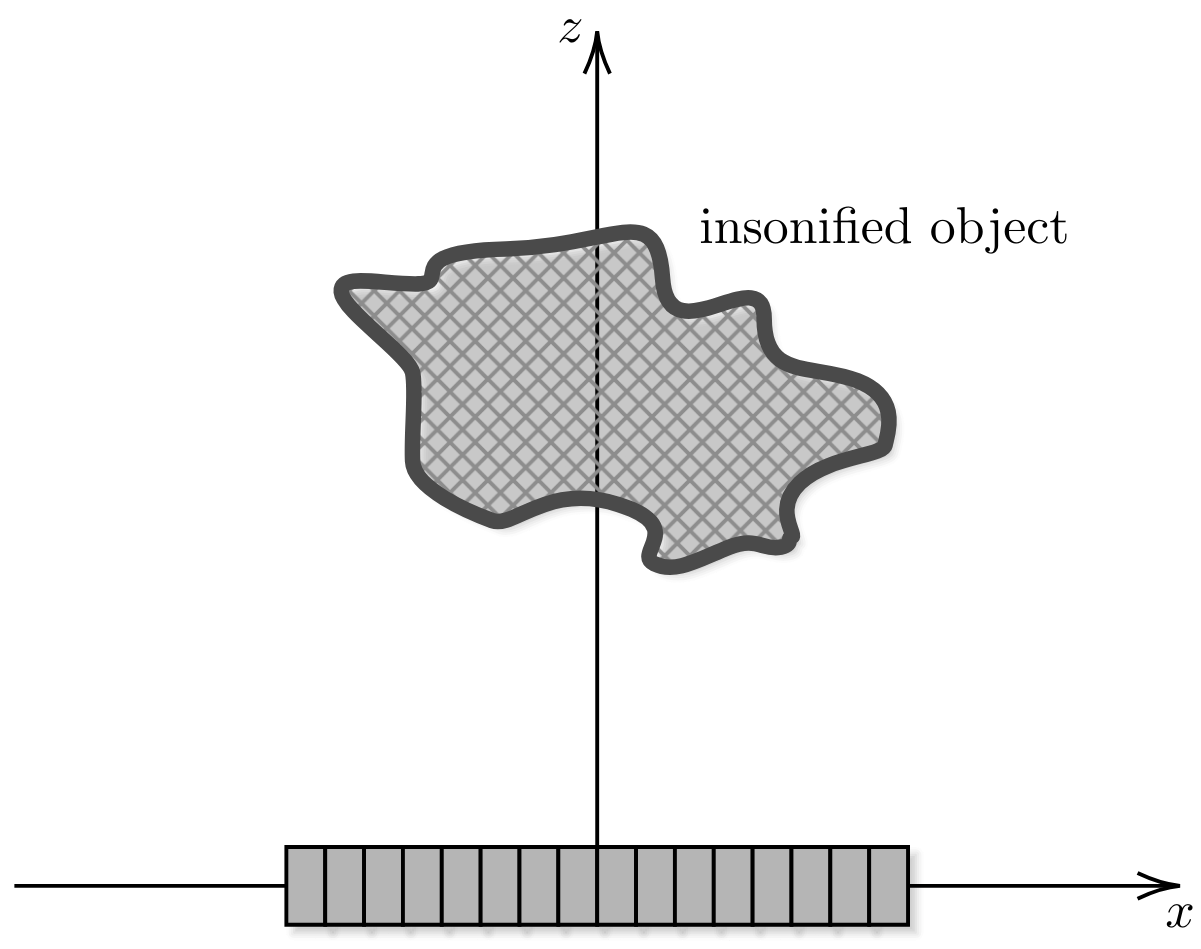
\includegraphics[width=0.5\textwidth]{images/array.png}
    \captionsetup{justification=centering}
    \caption{Sender/receiver array for ultrasound imaging \cite{Dorausch_2022}}
    \label{fig:us_array}
\end{figure}

The algorithm used for this k-space analysis is the \ac{fbi} proposed by Dorausch et al. This paper consists of three main parts the Fourier transformation into the k-space, the reconstruction of the image with the transformed data and the back transformation to get the final image. As it is important for an clinical ultrasound device the algorithm was investigated for its real time capability. In his bachelor thesis Richter \cite{Richter_2024} compared the implementation of this algorithm on different hardware. Once on a \ac{cpu} and once of the \ac{gpu} of a Snapdragon processor. For the analysis on an mobile processor synthetic data for 16 sender and 128 receiver was used. In figure \ref{fig:fft_an} it is shown that the \ac{fft} exceeds the realtime goal of 30 ms for a steady video output by approximately 10 times even with the implementation on a \ac{gpu}. It becomes clear that the \ac{fft} is the bottleneck for a realtime implementation of the image reconstruction algorithm. Therefore an efficient implementation of a large \ac{fft} is needed. The requirements for such an algorithm are discussed in the next chapter\cite{Dorausch_2022}.

\section{Realtime requirements} \label{sec:req}
As the algorithm proposed in this work should contribute to an image with the maximum possible quality some of the requirements are higher than in previous work. The goal of this thesis is to enable the realtime capability of an \ac{fft} algoritm for a system with 256 receivers and 10 senders. A property of the \ac{fbi} algorithm is that the use of longer signals leads to better imaging results. A sufficient length for this signal is 4 ms \cite{dorausch_adoption_2023}. Each of the 256 receivers records the reflection of this signal. The analogue signal is then sampled with an \ac{adc} with a sampling rate of 65.536 MHz and a resolution of 16 bit for one datapoint. This results in a $2^{18}$ datapoint \ac{fft} with 16 bit datapoints for every receiver. If again 30 ms goal for a steady 30 frames per second video stream is assumed, this means that 256 $2^{18}$ \ac{fft}s need to be done within 30 ms.

\begin{figure}[h!]
    \centering
    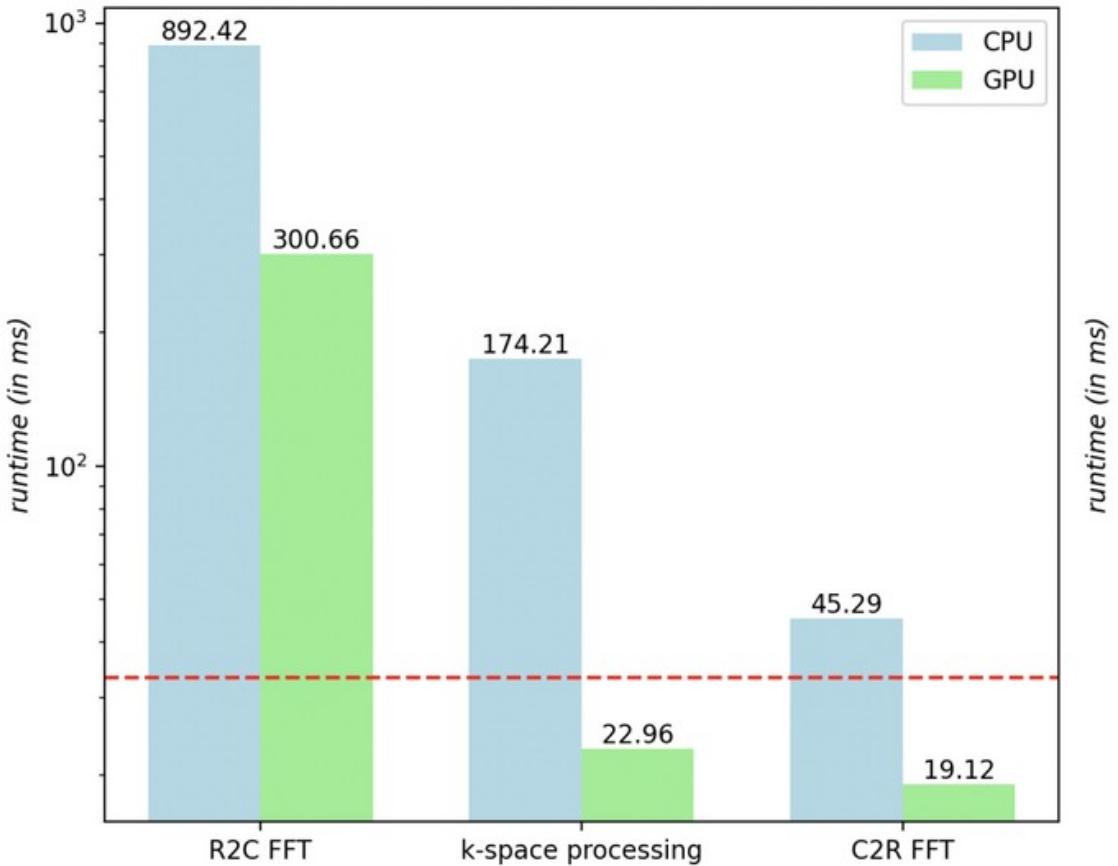
\includegraphics[width=0.4\textwidth]{images/fft_an.png}
    \captionsetup{justification=centering}
    \caption{Different parts of the \ac{fbi} algorithm by runtime and hardware \cite{Richter_2024} }
    \label{fig:fft_an}
\end{figure}

\section{Fast Fourier Transform}\label{sec:ft}
The Fourier transform is a foundational tool in digital signal processing, essential for analyzing the frequency components of signals. Fundamentally, it decomposes a signal into a set of sinusoids, each with a unique frequency, amplitude, and phase. This decomposition is typically implemented via the \ac{dft} or its efficient computation, the \ac{fft}. Equation \ref{eq:fft} shows the \ac{dft} \cite{muller_fundamentals_2015}.\par

\begin{equation}\label{eq:dft}
    X(k) = \sum_{n=0}^{N} x(n) e^{\frac{-2\pi i k n}{N}}\
\end{equation}

For real-time capability of the Discrete Fourier Transform, not only in Fourier-based imaging but 
also in other scenarios, fast computation is essential. One of the most renowned algorithms for 
achieving this is the Cooley-Tukey \ac{fft} algorithm. This algorithm significantly reduces the computational complexity 
of the \ac{dft} from \(O(n^2)\) to \(O(n \log n)\) using a divide-and-conquer approach, where the 
problem size is reduced for each computation. The main concept behind the Cooley-Tukey algorithm 
is to reduce the computational complexity of the \ac{dft} by exploiting symmetries and factoring the \ac{dft} 
into smaller components, which significantly decreases the number of operations needed. 
This design also allows for parallel computation, as not all operations depend on one 
another anymore \cite{cooley_algorithm_1965}.\par
To understand the construction of the Cooley-Tukey algorithm, it's best to begin with the radix-2 
case. The name stems from decomposing a \ac{dft} of length \(N\) into two interleaved \ac{dft}s with sizes 
\(N/2\). The initial step of this decomposition involves splitting the \ac{dft}, as defined in 
equation \ref{eq:dft}, into a sum of the even-indexed parts and the odd-indexed parts for 
\(k = N/2 - 1\).

\begin{equation}\label{eq:dft_even_odd}
    X(k) = \sum_{m=0}^{N/2 - 1} x(2m) e^{\frac{-2\pi i}{N} (2m) k} + \sum_{m=0}^{N/2 - 1} x(2m+1) 
    e^{\frac{-2\pi i}{N} (2m+1) k}\
\end{equation}

The multiplier \(e^{\frac{-2\pi i k}{N}}\) can be factored out, as shown in equation 
\ref{eq:even_odd_e}. This representation makes it clearer that the first \(N/2\) entries of the 
\ac{dft} are obtained by computing the \ac{dft} over the even-indexed parts and the \ac{dft} over the odd-
indexed parts separately. These results are then combined into an output vector, where the odd-
indexed parts are adjusted by the factors \(e^{\frac{-2\pi i k}{N}}\), known as the twiddle 
factors \cite{duhamel_fast_1990}.

\begin{equation}\label{eq:even_odd_e}
    X(k) = \sum_{m=0}^{N/2 - 1} x(2m) e^{\frac{-2\pi i}{N/2} mk} + e^{\frac{-2\pi i k}{N}} 
    \sum_{m=0}^{N/2 - 1} x(2m+1) e^{\frac{-2\pi i}{N/2} mk}\
\end{equation}

The calculation for the second \(N/2\) entries follows a similar pattern, as shown in equation 
\ref{eq:second_m}. The key distinction lies in the common multiplier factored out, which is 
\(e^{\frac{-2\pi i}{N}  (k + \frac{N}{2})}\). Due to the periodicity of \(e\), this is equivalent 
to \(-e^{\frac{-2\pi i k}{N}}\), as illustrated in equation \ref{eq:second_m_s}.

\begin{equation}\label{eq:second_m}
    X(k + \frac{N}{2}) = \sum_{m=0}^{N/2 - 1} x(2m) e^{\frac{-2\pi i}{N} (2m) (k + \frac{N}{2})} + 
    \sum_{m=0}^{N/2 - 1} x(2m+1) e^{\frac{-2\pi i}{N} (2m+1) (k + \frac{N}{2})}\
\end{equation}

\begin{equation}\label{eq:second_m_s}
    X(k + \frac{N}{2}) = \sum_{m=0}^{N/2 - 1} x(2m) e^{\frac{-2\pi i}{N/2} mk} - e^{\frac{-2\pi i 
    k}{N}} \sum_{m=0}^{N/2 - 1} x(2m+1) e^{\frac{-2\pi i}{N/2} mk}\
\end{equation}

Designating the even indexed \ac{dft} as \(E_{k}\) and the odd indexed \ac{dft} as \(O_{k}\), the entire \ac{dft} 
can be expressed in the form of the following two equations:

\begin{equation}\label{eq:even_dft}
    X(k) = E_{k} + e^{\frac{-2\pi i k}{N}} O_{k}\
\end{equation}

\begin{equation}\label{eq:odd_dft}
    X(k + \frac{N}{2}) = E_{k} - e^{\frac{-2\pi i k}{N}} O_{k}\
\end{equation}

In these equations, the final results are obtained by combining the two \ac{dft}s \(E_{k}\) and 
\(O_{k}\) through a +/- operation. This addition for the even parts and subtraction for the uneven parts, 
commonly referred to as a butterfly, is itself a \ac{dft}. With this understanding, a more general form of the 
\ac{fft} algorithm can be derived, where the butterfly operation is not limited to inputs of two. Instead, 
larger \ac{dft}s can be used to combine the results, with the size often referred to as the radix, describing 
the resulting combining \ac{dft} \cite{muller_fundamentals_2015}.\par
This implies that a large \ac{dft} of size \(N\) can be decomposed into two smaller \ac{dft}s of sizes 
\(N_{1}\) and \(N_{2}\), where \(N = N_{1} * N_{2}\). In this scenario, \(N_{1}\) \ac{dft}s of size 
\(N_{2}\) would be performed first. The results of this stage would then be combined with 
\(N_{2}\) \ac{dft}s of size \(N_{1}\). This generalization can be expressed in the following equation:

\begin{equation}\label{eq:fft}
    X(k) = \sum_{n_{1} = 0}^{N_{1} - 1} e^{\frac{-2\pi i}{N_{1} N_{2}}n_{1}k_{2}} (\sum_{n_{2} = 0}
    ^{N_{2} - 1} x_{N_{1}n_{2}+n_{1}} e^{\frac{-2\pi i}{N_{2}}n_{2}k_{2}}) e^{\frac{-2\pi i}{N_{1}}
    n_{1}k_{1}}
\end{equation}


One crucial aspect of this algorithm is its potential for recursive application. All smaller \ac{dft}s 
can be addressed by the Cooley-Tukey algorithm itself and decomposed into even smaller \ac{dft}s. This 
recursive approach leads to the notion that a decomposition is the radix \(X\) of an \ac{fft}, meaning 
that all \ac{dft}s larger than \(X\) are successively reduced until they reach the size of \(X\).\par
Moreover, it is feasible to employ mixed radix decomposition, incorporating different radices at 
various stages of the \ac{fft}. This results in multiple possible decompositions of a single \ac{dft} 
\cite{qureshi_generation_2011}. The primary differences between these variants lie in the level of 
parallel transforms and the complexity of the twiddle factors. This complexity can be 
advantageous, as periodicity of the twiddle factors can lead to simplifications. While many of 
these simplifications may not be of significant mathematical interest, they play a crucial role in 
hardware implementation. Determining which simplifications are essential depends on understanding 
the underlying hardware. Consequently, the next section will provide an overview of the hardware 
utilized in this thesis.
%TODO one paragraph for comparison with \ac{dft}2d


%TODO adopt this whole section
\section{Versal Adaptive Computer Acceleration Platform}\label{sec:versal}
The hardware basis for this thesis is the VCK190 evaluation board with the VC1902 Adaptive Computer 
Acceleration Platform (ACAP), developed by Xilinx. The ACAP is a heterogeneous \ac{soc}
comprising multiple integrated hardware components and user-programmable hardware designs. All of these 
components are interconnected via a \ac{noc}. The network employs an AXI4 network, 
implemented outside the configurable logic blocks, which frees up resources. The hardware components 
dedicated to computing can be divided into three main categories. As illustrated in figure 
\ref{fig:high_scheme}, the aforementioned main components can be classified into three categories: 
scalar engines, adaptable engines and intelligent engines \cite{AMD_a_aie}.\par

\begin{figure}[h]
    \centering
    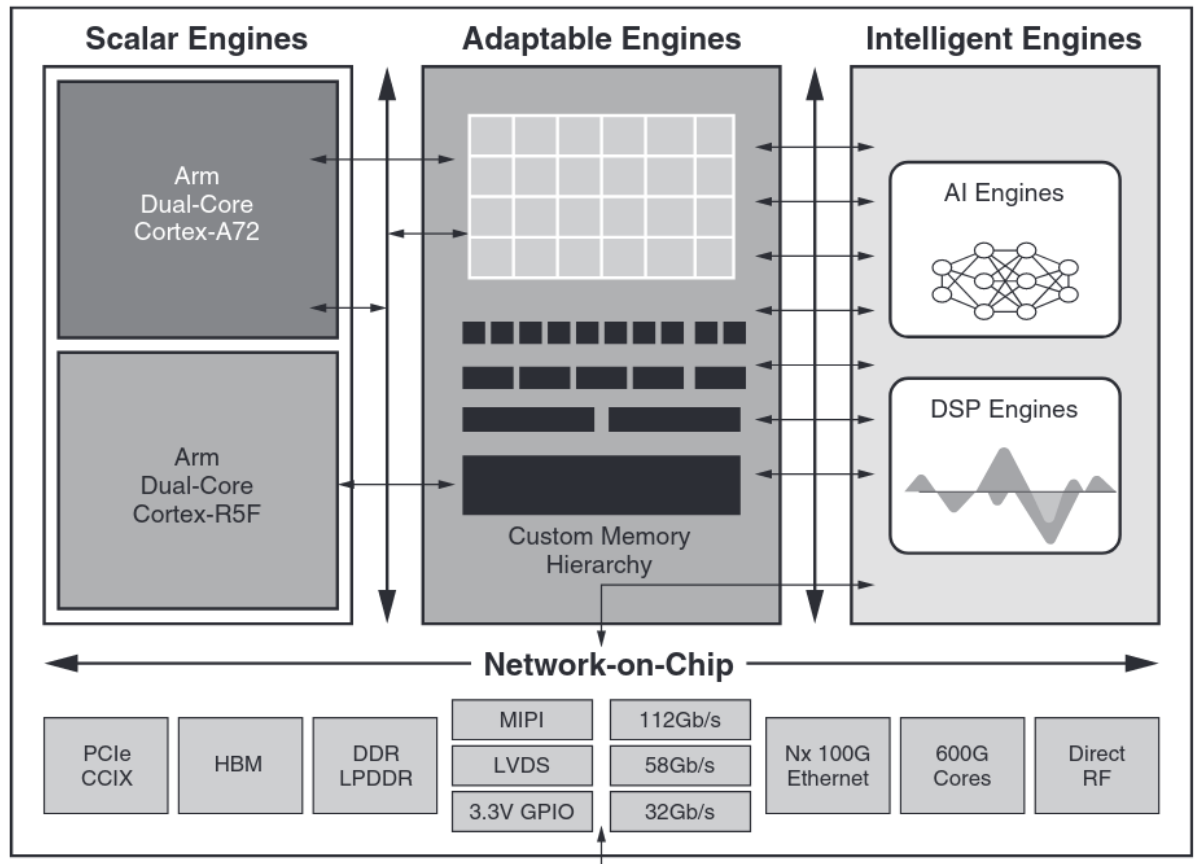
\includegraphics[width=0.6\textwidth]{images/high_level_vc1902.png} %adopt font and textsize
    \captionsetup{justification=centering}
    \caption{Overview of the VC1902 \cite{AMD_a_aie}}
            Highlevel view of the VC1902 which shows the three main parts which are connected via a \ac{noc}. Shows also some of the peripheral elements like Ethernet and memory controller
    \label{fig:high_scheme}
\end{figure}

\subsection{Scalar Engines}
The scalar engines are composed of the ARM-Cortex-A72 CPU and an ARM-Cortex-R5F real-time CPU. In 
conjunction with peripheral components, including USB, UART and PCIe controllers, they constitute the 
processing system (PS). This system is connected to the DDR memory controller via the \ac{noc}, which allows 
the sharing of this controller with the \ac{pl}. In an embedded system, the primary 
function of the processing system is to serve as a host for other system components. The software is 
executed and specific hardware-optimised components are delegated to the adaptable engines or 
intelligent engines. The ARM cores permit either the execution of bare-metal applications for this 
scenario or the hosting of a full operating system, which allows the user to take advantage of the 
system's features and usermode libraries for interaction with the \ac{pl}. In this work, the 
latter case is employed with the Petalinux operating system, developed by Xilinx for their boards. This 
enables the use of the Xilinx runtime environment (XRT) to interact with the adaptable engines and 
intelligent engines, thereby facilitating the utilisation of special libraries to reduce the 
development overhead associated with existing software and hardware features \cite{AMD_a_aie}.

\subsection{Adaptable Engines}
The term "programmable logic" is used to describe the adaptable engines. The system comprises 
configurable logic blocks (CLBs), internal memory, and digital signal processing (DSP) engines. It can 
be considered an \ac{fpga} like structure that enables the processing of irregular data. The CLBs utilise 
the conventional design of look-up tables (LUTs) and flip-flops. The internal memory of the \ac{pl} 
comprises 967 block-RAM elements, each of which can store 36 kilobytes of data, and 463 ultra-RAM 
elements, which can hold 288 kilobytes of memory each. To enhance flexibility, the \ac{pl} is partitioned 
into multiple clock regions. Typically, such regions contain 24 block and ultra-RAM elements. In order 
to transfer data between \ac{pl} endpoints, the \ac{noc} is employed. This is typically done via the PS or other 
integrated blocks. The NoC can be employed to free resources in the \ac{pl} that would otherwise be used for 
routing, thus facilitating communication between different \ac{pl} endpoints. The connection to the NoC can 
be configured with AXI3, AXI4, or AXI4 Stream. The NoC employs a 128-bit-wide NoC packet protocol 
internally \cite{AMD_a_aie}.\par

\begin{figure}[h]
    \centering
    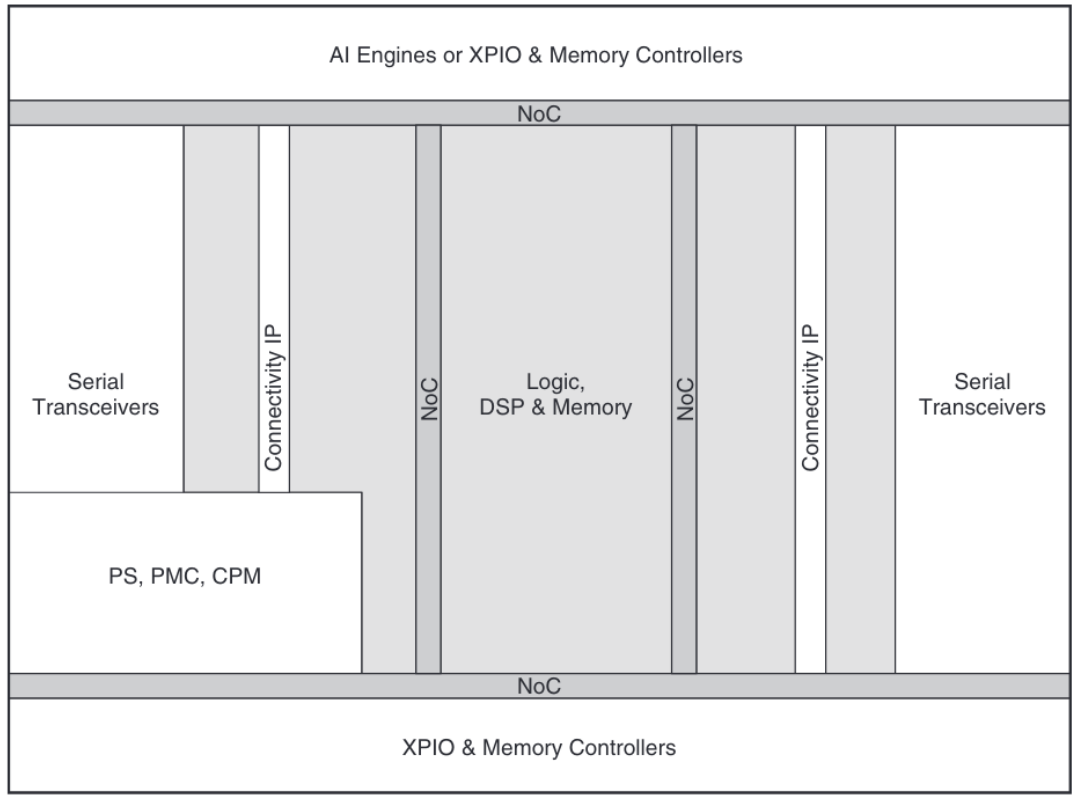
\includegraphics[width=0.6\textwidth]{images/low_level_vc1902.png}
    \captionsetup{justification=centering}
    \caption{Schematic of the VC1902 chip design \cite{AMD_a_aie}}
            Deeper look into the organisation of the three main components. It is shown that this elements are much more integrated than shown in previous schematics. 
    \label{fig:low_scheme}
\end{figure}

\subsection{Intelligent Engines}
The intelligent engines comprise digital signal processors (DSP) elements and artificial intelligence 
(AI) engines. The DSP elements are not formally part of the intelligent engines. As illustrated in 
figure \ref{fig:low_scheme}, the DSP elements are situated within the \ac{pl}. This is due 
to the structure of such an DSP element, which consists of a 27-bit pre-adder, a 27x28 multiplier, and 
a 48-bit arithmetic logic unit (ALU), as illustrated in figure \ref{fig:dsp}. Additionally, it 
comprises a multitude of registers for the storage of input values and results. In order to optimise 
the utilisation of these elements, it is necessary to employ the use of memory, such as block RAM, 
which must be directly connected to the element in question. Another crucial aspect of placing these 
elements in a \ac{pl} is the capability to cascade operations through multiple DSP elements. 
This is made possible through the CARRYCASCIN and CARRYCASCOUT pins. Furthermore, single instruction 
multiple data (SIMD) operations are made available. In conjunction with cascading two 24-bit SIMD 
accumulators or four 12-bit SIMD accumulators, the aforementioned elements can be employed. 
Furthermore, the internal MULTSIGNIN and MULTSIGNOUT cascade signals permit the utilisation of 96-bit 
multiply-accumulate (MAC) operations \cite{AMD_a_aie}.\par

\begin{figure}
    \centering
    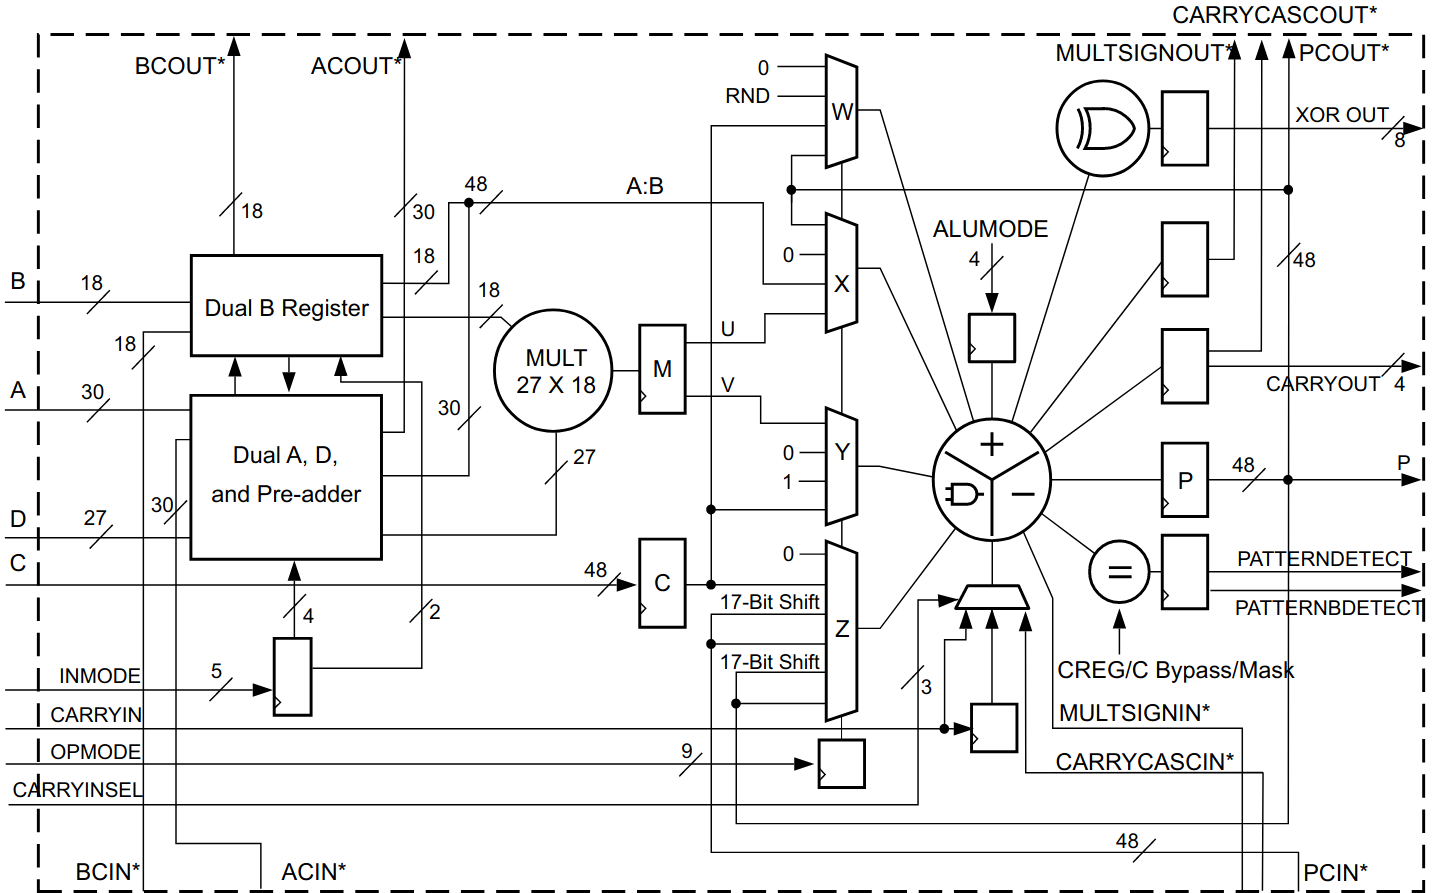
\includegraphics[width=0.7\textwidth]{images/dsp_detail.png}
    \captionsetup{justification=centering}
    \caption{Detailed schematic of the DSP Slice \cite{AMD_a_aie}}
            The interconnection between multiplexer, adder and multiplication units within the DSP is shown. Additional single bit lane are highlighted to show potential cascade connections.
    \label{fig:dsp}
\end{figure}

\subsubsection{AI Engines}
Another essential component of the intelligent engines is the AI Engine array, comprising newly developed AI accelerators, as previously mentioned. The VCK190 platform includes 400 of these engines, arranged in a two-dimensional tile array. This array is connected to \ac{pl} through eight specialized connection tiles, supporting the AXI standard \cite{AMD_a_aie}.\par

\begin{figure}[h!]
    \centering
    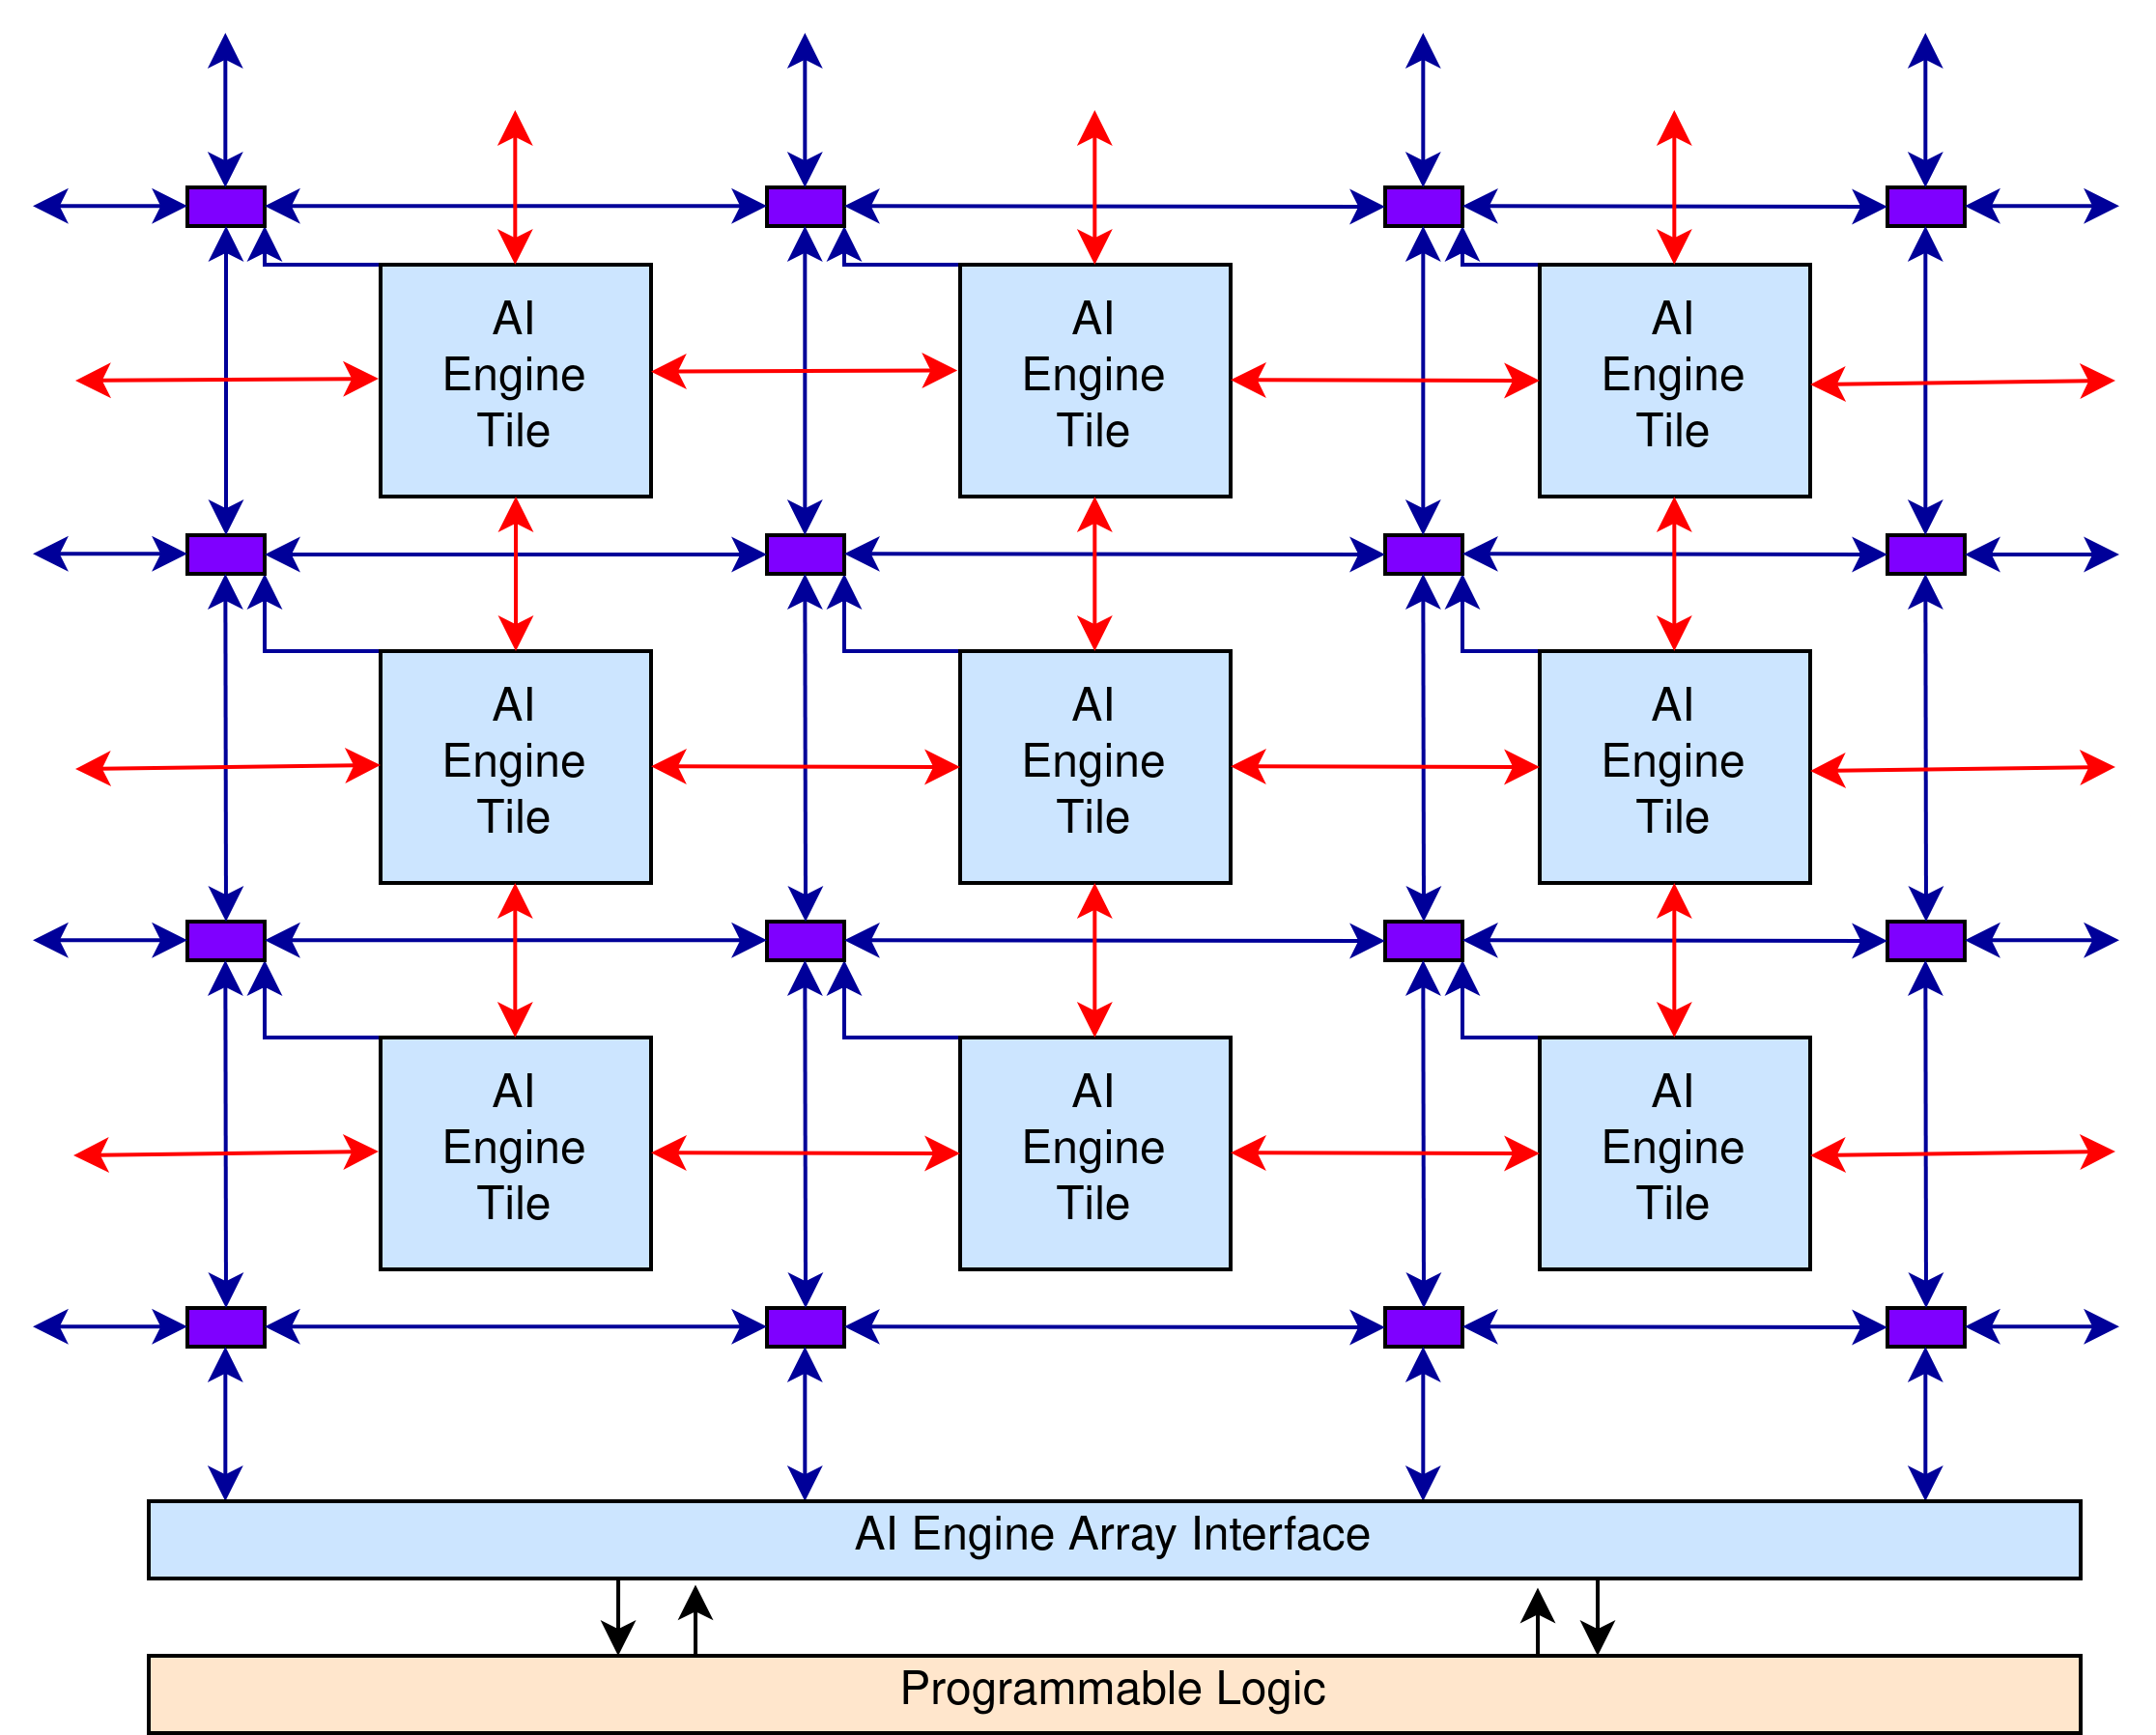
\includegraphics[width=0.7\textwidth]{images/ai_array.png}
    \captionsetup{justification=centering}
    \caption{AI Engine array}
            A schematic that shows the AI Engine array with its different connections. Red connections between the tiles show the direct memory access between tiles while purple shows the streaming interface between further away tiles. At the bottom of the array the interface to the PL is shown \cite{AMD_a_aie}.
    \label{fig:ai_array}
\end{figure}

As depicted in figure \ref{fig:ai_array}, each tile in the array is interconnected, featuring two primary types of communication pathways. The first is an AXI-based network connecting all tiles. This network facilitates data transmission among the tiles via a routing and switching system that can split or merge multiple data streams. Specifically, the network can divide a single stream into up to 32 sub-streams or merge up to 32 sub-streams back into a single stream. This stream management is enabled by data packet headers, which identify the respective substream for routing.\par
The second type of connection provides direct access between adjacent tiles, where each tile can access the memory of its neighboring tiles to the north, south, east, and west. This arrangement allows for efficient memory usage and reduces memory overhead, particularly when two accelerators require shared memory access.\par
To provide a deeper understanding of this technology, the specific structure of the tiles is outlined in detail. As illustrated in figure \ref{fig:detail_tile}, each tile contains the aforementioned memory and an AI Engine core, which serves as the primary accelerator. This memory comprises 32 KB, divided into eight 8 KB banks, each accessible in parallel by the streaming interfaces. As noted earlier, this memory can also be accessed by neighboring AI Engine cores on adjacent tiles \cite{AMD_aie_k}.\par

\begin{figure}[h!]
    \centering
    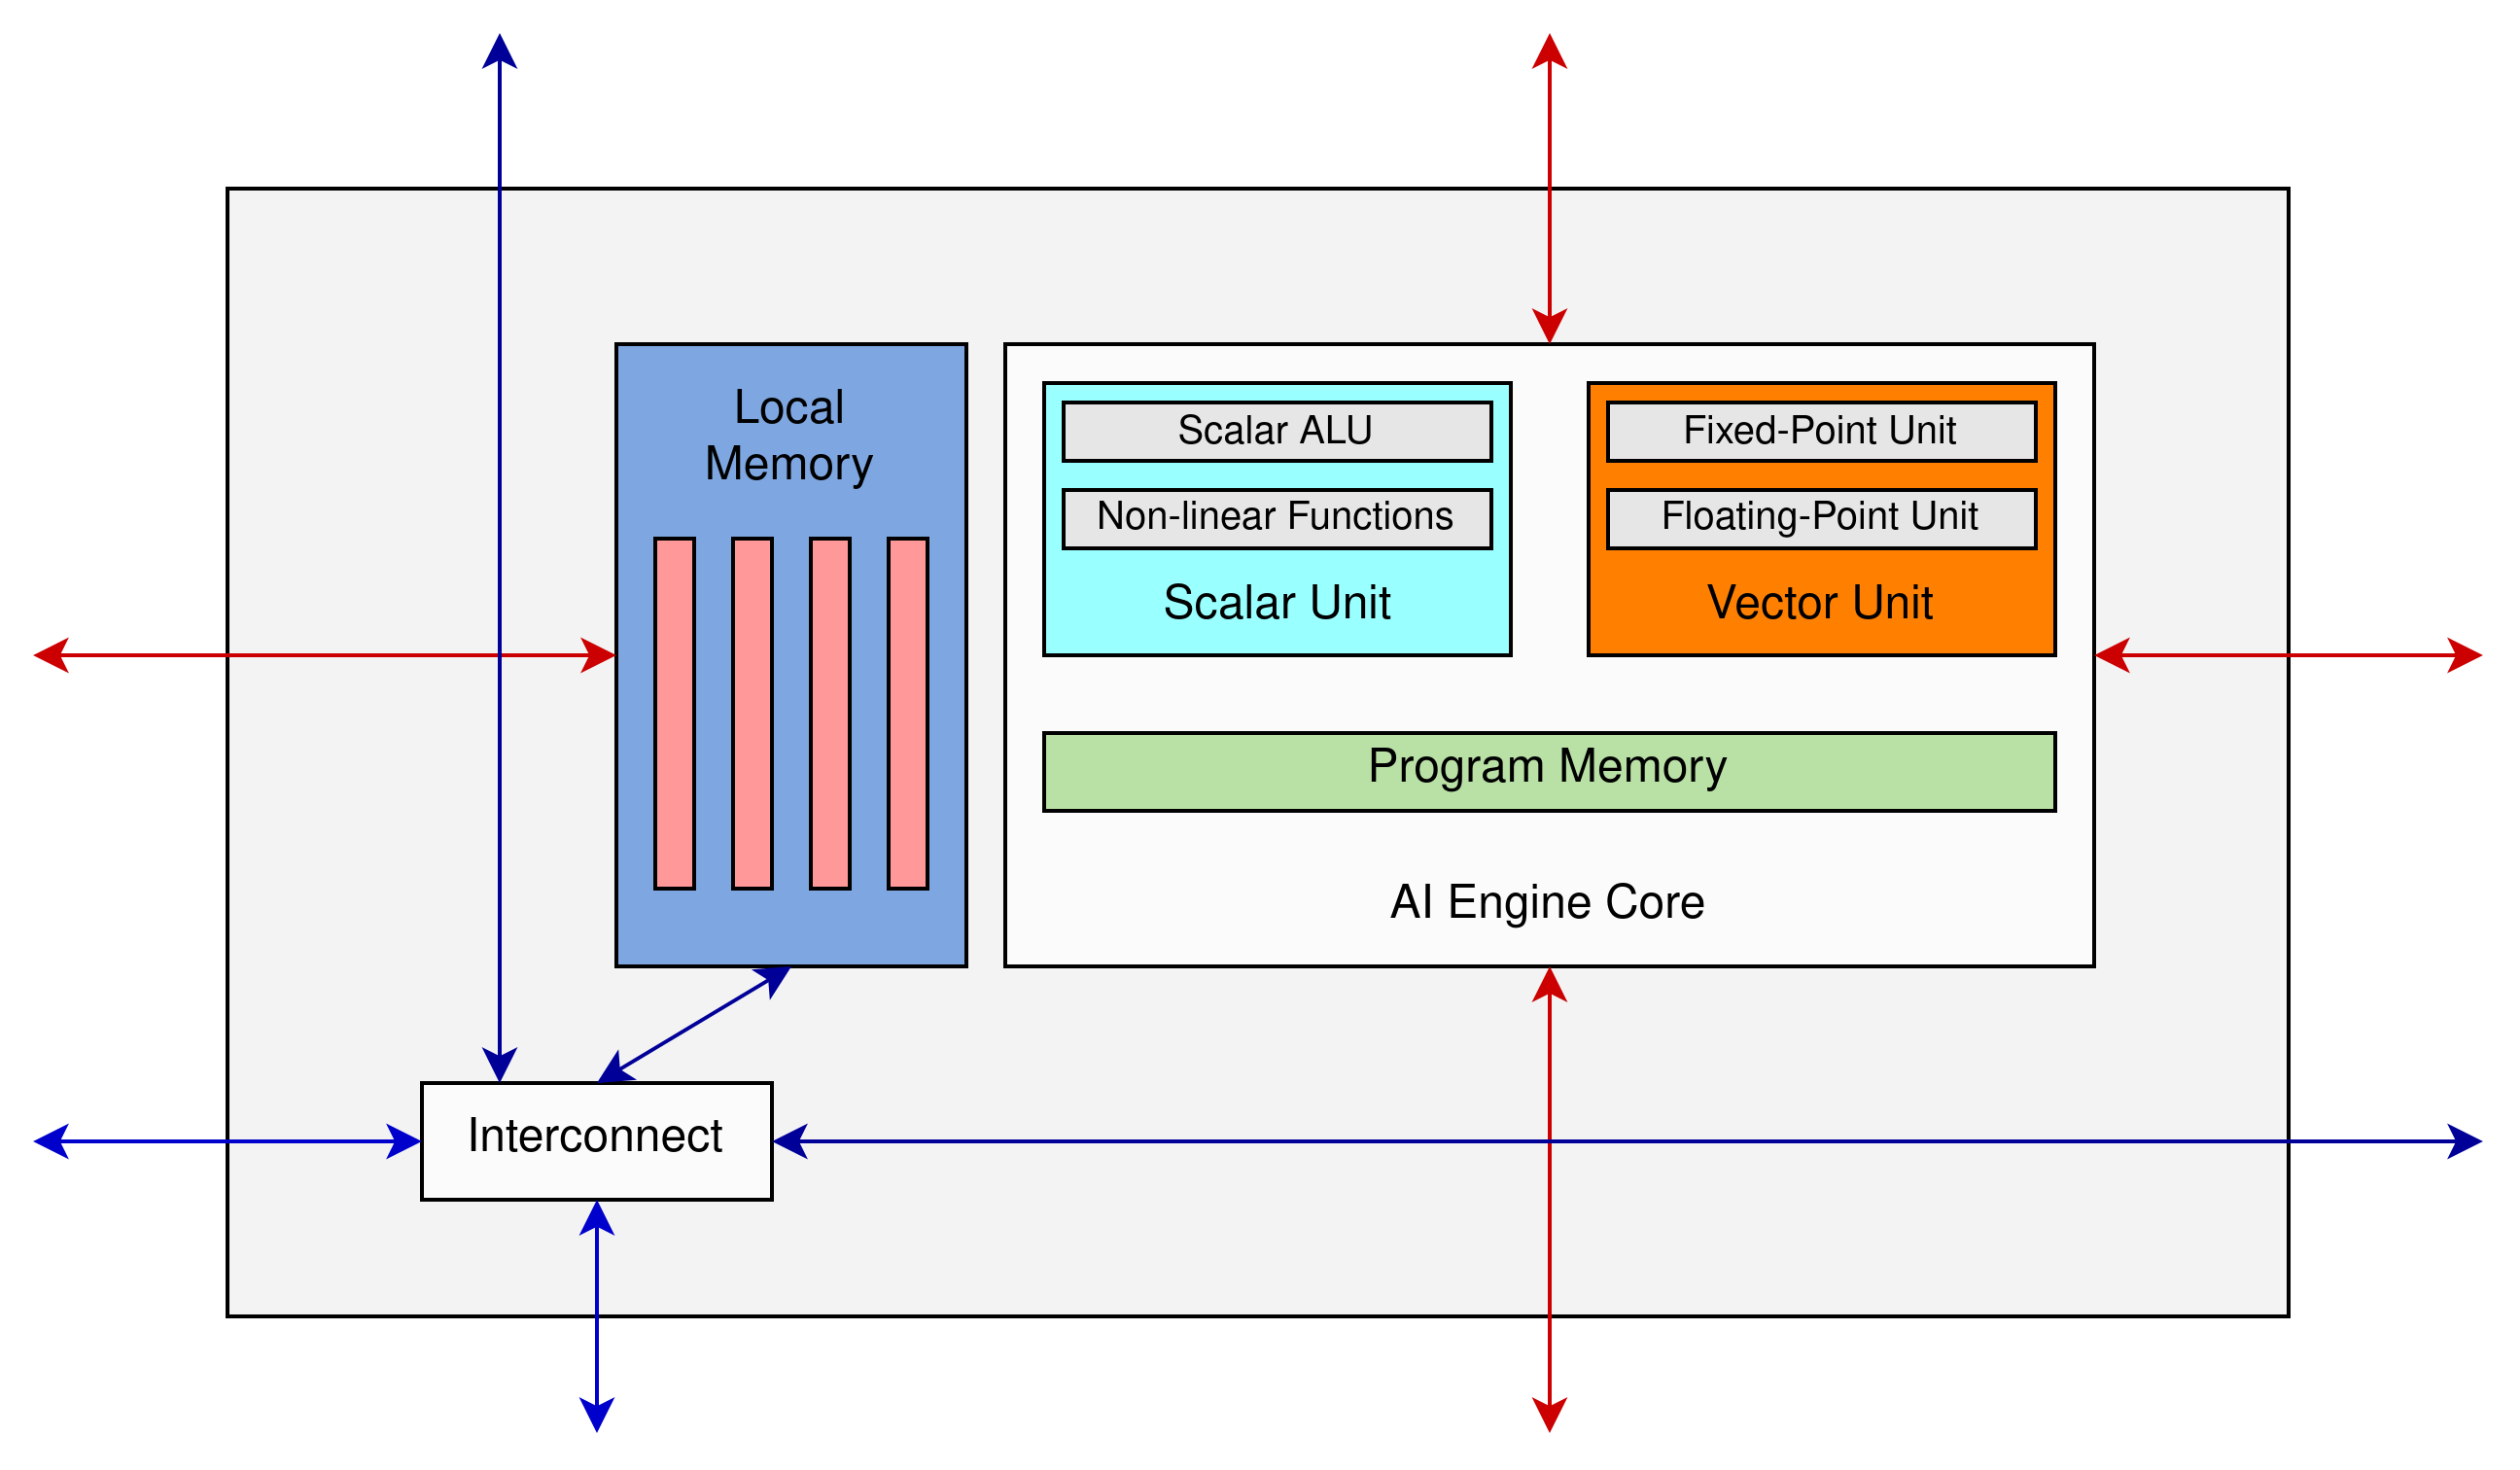
\includegraphics[width=0.9\textwidth]{images/detail_tile.png}
    \captionsetup{justification=centering}
    \caption{AI Engine tile}
            Detailed look into the AI Engines with the different component of the core. The four local memory banks of the core are shown in red, the different calculation units of the RISC processor are shown in blue (scalar) and orange (vector). Connections to the other tiles within the array are also highlighted. 
    \label{fig:detail_tile}
\end{figure}

The AI Engine core itself is a compact \ac{risc} processor equipped with 16 KB of dedicated program memory, as well as one scalar and one vector processing unit. The vector unit's register structure is depicted in the table \ref{tab:reg}. At the hardware level, the vector unit includes 16 registers, each 128 bits wide, which can be combined to form larger registers as needed. These registers can be addressed directly via a dedicated storage directive, utilizing the register names specified in the figure. This registers can be accessed with special functions so called intrinsics . They allow fine grained access to this registers and enable to full use of the vector unit \cite{AMD_aie_intrinsics, AMD_a_aie_s}.\par

\begin{table}
\centering
\resizebox{0.4\textwidth}{!}{
\begin{tblr}{
  cells = {c},
  cell{1}{4} = {c=2}{},
  cell{2}{2} = {r=2}{},
  cell{2}{3} = {r=4}{},
  cell{2}{4} = {r=8}{},
  cell{2}{5} = {r=4}{},
  cell{4}{2} = {r=2}{},
  cell{6}{2} = {r=2}{},
  cell{6}{3} = {r=4}{},
  cell{6}{5} = {r=4}{},
  cell{8}{2} = {r=2}{},
  cell{10}{2} = {r=2}{},
  cell{10}{3} = {r=4}{},
  cell{10}{4} = {r=4}{},
  cell{10}{5} = {r=4}{},
  cell{12}{2} = {r=2}{},
  cell{14}{2} = {r=2}{},
  cell{14}{3} = {r=4}{},
  cell{14}{4} = {r=4}{},
  cell{14}{5} = {r=4}{},
  cell{16}{2} = {r=2}{},
  vlines,
  hline{1-2,10,14,18} = {-}{},
  hline{3,5,7,9,11,13,15,17} = {1}{},
  hline{4,8,12,16} = {1-2}{},
  hline{6} = {1-3,5}{},
}
128-bit & 256-bit & 512-bit & 1024-bit &              \\
vrl0    & wr0     & xa      & ya       & N/A          \\
vrh0    &         &         &          &              \\
vrl1    & wr1     &         &          &              \\
vrh1    &         &         &          &              \\
vrl2    & wr2     & xb      &          & {yd\\(msbs)} \\
vrh2    &         &         &          &              \\
vrl3    & wr3     &         &          &              \\
vrh3    &         &         &          &              \\
vcl0    & wc0     & xc      & N/A      & N/A          \\
vch0    &         &         &          &              \\
vcl1    & wc1     &         &          &              \\
vch1    &         &         &          &              \\
vdl0    & wd0     & xd      & N/A      & {yd\\(lsbs)} \\
vdh0    &         &         &          &              \\
vdl1    & wd1     &         &          &              \\
vdh1    &         &         &          &              
\end{tblr}
}
\caption{Vector registers of the vector unit \cite{AMD_aie_intrinsics}}
        The addressing scheme for the vector registers. Each column shows a different addressing scheme for different data width of the registers.
\label{tab:reg}
\end{table}

The initialization of the AI engines occurs during boot-up, and configurations cannot be altered during runtime. The code designated for each engine is compiled and loaded into the 16 KB program memory. Data flow between engines is organized in a predefined graph, which establishes routing information across the network connecting individual tiles. This graph is also initialized during boot-up.\par
Following initialization, the AI engines are managed through either the Scalar Engines or \ac{pl} using a target offloading approach. Data is transferred into the AI engine array for processing, after which it exits via the connection tiles in an AXI stream format. The \ac{pl} then either processes this data directly or writes it to the chip’s DDR memory, signaling the ARM host processor for further handling. The entire array operates at a fixed clock rate of 1250 MHz.

\chapter{Related Work}
%It must be clear what is being worked on elsewhere. Especially the gaps of the others should be made clear. Why is your own work, your own approach important in order to advance the state of the art? This chapter is ignored by many readers (but not by the reviewer ;-), also later in publications "Related Work" is an important thing. (5-15 pages)
The efficient implementation of the Fourier Transform is by no means an unknown problem. Because many analysis in signal processing relies on it there are various approaches 
for implementations. Most of them come from the radar filed and deal with less antennas and with a smaller density in reflected waves. Therefore the amount of data points which are recorded are less than in the ultra sound setup of this work. These approaches still yield valuable insides into how to construct a fast and efficient \ac{fft}. Therefore this chapter will give an overview over the previous work and discuss some downsides for the use case of this work.

%TODO citation for this section
\section{Effectiveness of FFT Implementations on GPU}
One potential component for executing large \ac{fft}s is the \ac{gpu}. Designed specifically for processing vast amounts of data, \ac{gpu}s can perform identical operations across multiple data points in parallel. This parallelization greatly benefits \ac{fft} implementations. As previously mentioned, the Cooley-Tukey approach divides the \ac{dft} into smaller segments, which can be processed concurrently. The functionality of a \ac{gpu} in this context operates as follows: data to be processed is first copied into the \ac{gpu}’s memory, where multiple processing units execute the same calculation on distinct subsets of the data. Modern \ac{gpu}s, specialized for this purpose, contain up to tens of thousands of these processing units. To utilize them, the program must partition the data into subsets and define a kernel, the specific calculation, to be applied to each subset. Research indicates that using a \ac{gpu} can significantly boost performance compared to a \ac{cpu}, with complete radix-2 \ac{fft} decompositions showing up to a 30-fold improvement in runtime \cite{puchala_effectiveness_2015}.\par
The primary limitation for \ac{gpu}-based \ac{fft}s, however, lies not in computational power but in memory bandwidth constraints during data exchanges with the \ac{cpu} \cite{lloyd_fast_2008}. All data must be transferred to the \ac{gpu}’s memory before processing and then copied back into the main memory afterward to enable further computations. This memory transfer overhead becomes an issue because the \ac{fft} is only one step in a larger image reconstruction process. One approach to address this limitation is to perform the entire \ac{fbi} algorithm on the \ac{gpu}. This was attempted by Richter, although it was restricted to smaller datasets. This restriction is critical because current \ac{fft} implementations on \ac{gpu}s allow for two main approaches. In the first, a large \ac{fft} is computed, but results must be copied back to main memory for further processing \cite{cufft}. In the second, \ac{fft}s are embedded within a larger computation, eliminating the need for repetitive data transfers. However, this approach currently only supports \ac{fft} sizes up to 256 points \cite{cufftdx}.\par
Thus, adapting the \ac{fbi} algorithm for \ac{gpu} use with larger datasets would require a new \ac{fft} implementation that accommodates more extensive data while minimizing memory transfers. Even with such an implementation, data would still need to be copied to the \ac{gpu}’s memory. An alternative solution is to use \ac{fpga}s, which can be directly connected to \ac{adc}s receiving data from sensors. The following section will explore \ac{fft} implementations on \ac{fpga}s as a potential solution to this challenge.

\section{Large FFT implementation on a single FPGA}
The paper "A 1 Million-Point FFT on a Single FPGA" by Hans Kanders et al. \cite{kanders_1_2019} focuses on the efficient hardware implementation of a large-scale \ac{fft} on a single \ac{fpga}, targeting a 1-million-point \ac{fft} computation. The key challenge addressed is optimizing the computational architecture to meet the high resource and performance demands of such a large \ac{fft}, while staying within the constraints of a single \ac{fpga} platform.\par

\begin{figure}[h]
    \centering
    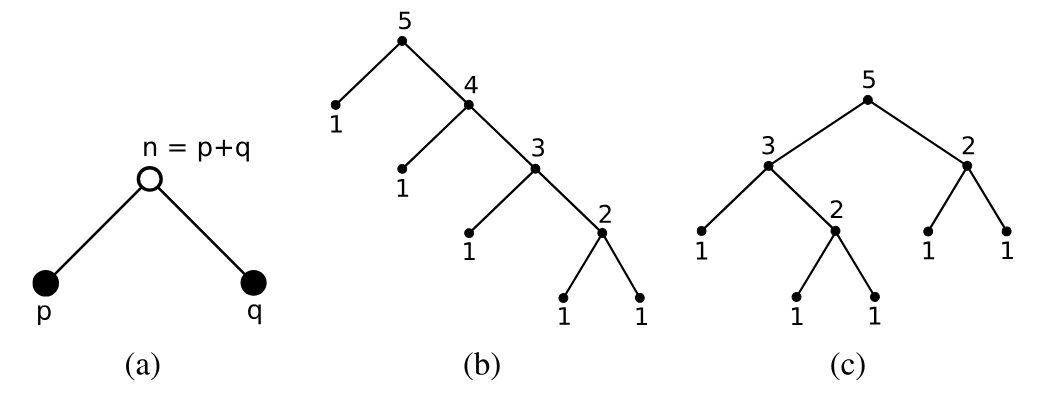
\includegraphics[width=0.7\textwidth]{images/trees.png}
    \captionsetup{justification=centering}
    \caption{Possible decompositions in tree form \cite{qureshi_generation_2011}}
            All of the possible decompositions of the FFT represented as powers of two as part of a tree.
    \label{fig:trees}
\end{figure}

The work especially explores the use of specific decomposition which would reduce the calculation effort. The various decompositions of the \ac{dft} a shown in a tree with the different smaller \ac{fft}s as powers of two (see figure \ref{fig:trees}). Implemented in hardware some of the phase rotations between the different stage become trivial for calculations as they turn out to be one or zero.  As the table in figure \ref{fig:rotator_table} shows various algorithm with different amounts of trivial rotators are possible. The rotators are shown as roots of unity were a larger number indicates a more complex calculation.  It is shown that larger rotators should be placed later in the algorithm has they demand a change in the data word length in the \ac{fpga} \cite{qureshi_generation_2011}.\par

\definecolor{Silver}{rgb}{0.752,0.752,0.752}
\definecolor{Gray}{rgb}{0.501,0.501,0.501}

\begin{table}
\centering
\resizebox{0.4\textwidth}{!}{
\begin{tblr}{
  cells = {c},
  cell{1}{2} = {c=3}{},
  cell{3}{2} = {Silver},
  cell{3}{3} = {Silver},
  cell{3}{4} = {Silver},
  cell{5}{3} = {Silver},
  cell{5}{4} = {Silver},
  cell{7}{3} = {Silver},
  cell{7}{4} = {Silver},
  cell{9}{3} = {Silver},
  cell{9}{4} = {Silver},
  cell{11}{2} = {Silver},
  cell{11}{3} = {Silver},
  cell{11}{4} = {Silver},
  cell{12}{2} = {Gray},
  cell{13}{2} = {Silver},
  cell{13}{3} = {Silver},
  cell{13}{4} = {Silver},
  cell{14}{3} = {Gray},
  cell{15}{3} = {Silver},
  cell{15}{4} = {Silver},
  cell{17}{3} = {Silver},
  cell{17}{4} = {Silver},
  cell{18}{2} = {Silver},
  cell{18}{4} = {Gray},
  cell{19}{3} = {Silver},
  cell{19}{4} = {Silver},
  cell{21}{2} = {Silver},
  cell{21}{3} = {Silver},
  cell{21}{4} = {Silver},
  vlines,
  hline{1-3,22-23} = {-}{},
  hline{4-21} = {2-4}{},
}
                    & Algorithm &         &         \\
Stage               & 10-20-10  & 12-20-8 & 16-20-4 \\
1                   & W4        & W4      & W4      \\
2                   & W8        & W16     & W16     \\
3                   & W32       & W4      & W4      \\
4                   & W4        & W256    & W256    \\
5                   & W1024     & W4      & W4      \\
6                   & W4        & W16     & W16     \\
7                   & W8        & W4      & W4      \\
8                   & W32       & W4096   & W65k    \\
9                   & W4        & W4      & W4      \\
10                  & W1M       & W16     & W16     \\
11                  & W4        & W4      & W4      \\
12                  & W8        & W1M     & W256    \\
13                  & W32       & W4      & W4      \\
14                  & W4        & W16     & W16     \\
15                  & W1024     & W4      & W4      \\
16                  & W4        & W256    & W1M     \\
17                  & W8        & W4      & W4      \\
18                  & W32       & W16     & W16     \\
19                  & W4        & W4      & W4      \\
{Trivial\\rotators} & 8         & 10      & 10      
\end{tblr}
} % Ende \resizebox
\caption{Algorithm variants with different decompositions \cite{kanders_1_2019}}
        Overview over the rotators of different decompositions as roots of unity. Trivial rotators are marked with light grey. The largest rotator is marked with dark grey.
\label{fig:rotator_table}
\end{table}

With this considerations in mind the 12-20-8 algorithm with two to the power of 4 or 5 as the smallest calculation unit is chosen. The algorithm is implemented into an \ac{fpga} using special units for the rotators. The design only uses up to 12 percent of calculation and I/O units but 67 percent of the memory units of the \ac{fpga}. This makes this approach as a solution for the large \ac{fft} for multiple channels insufficient as the run time is with 0.5ms above the maximum run time of 0.11 ms. Due to the high memory requirements it is not possible to run the whole algorithm in parallel to make up for the long run time \cite{kanders_1_2019}.

\section{Block-by-Block Configurable Fast Fourier Transform}
In a white paper Xilinx engineers describe a way to implement a 4096 datapoint \ac{fft} with little space consumption on the AI Engines. This approach stands out due to its ability to adjust the size and configuration of the \ac{fft} depending on the specific requirements of a given task. The \ac{fft} is therefore split into multiple building blocks, hence the name block-by-block configurable \ac{fft}. This blocks represent smaller \ac{fft}s due to a split up according to the Cooley-Tukey algorithm. In figure \ref{fig:packet_array} this decomposition is shown. The grey boxes represent one AI Engine tile there. All of the \ac{fft} blocks can be configured for a certain transform size by an control word. To get data to these blocks the implementation uses a combination of an AXI stream and the AI Engines packet switching. For the calculation int32 values are used to save up memory for precalculated twiddle factors \cite{block_by_block}.\par

\begin{figure}[h]
    \centering
    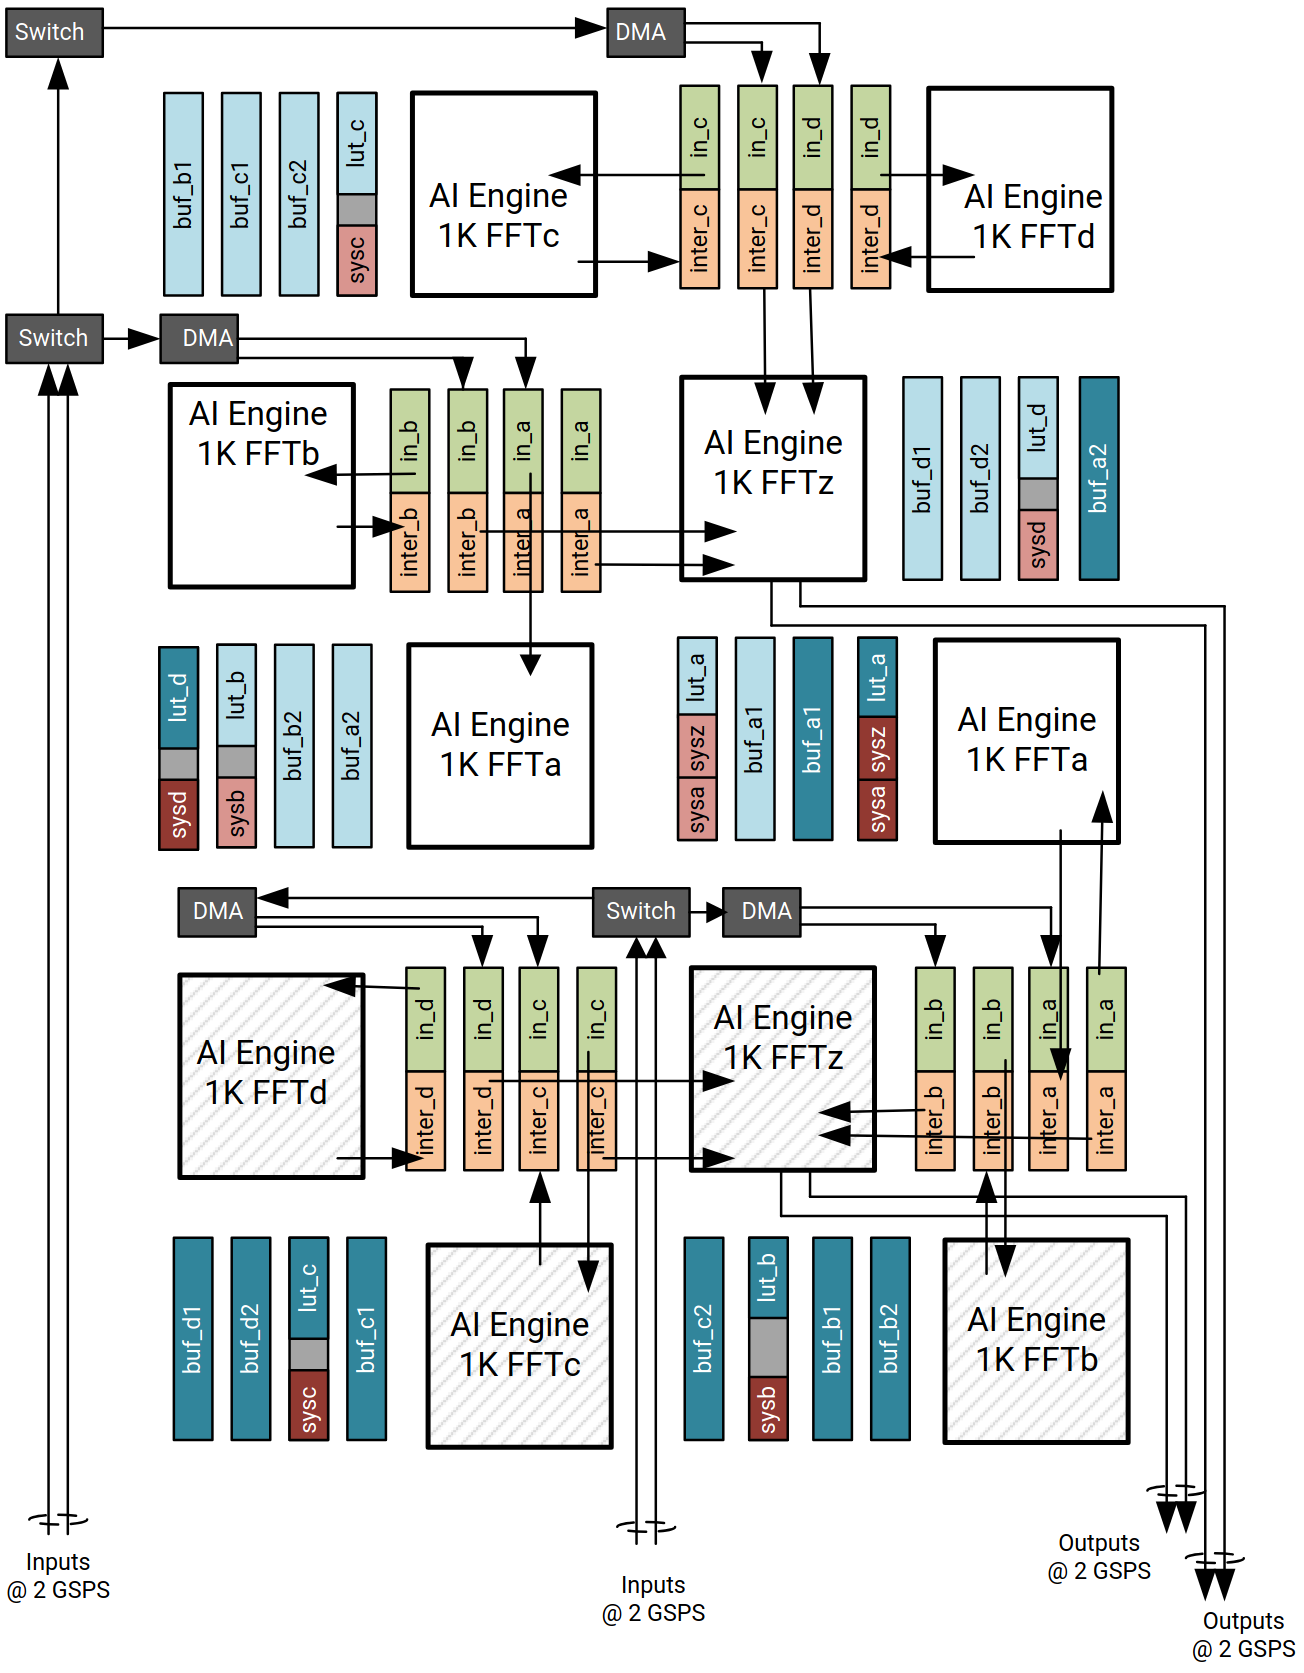
\includegraphics[width=0.65\textwidth]{images/packet_array.png}
    \captionsetup{justification=centering}
    \caption{Two of the described modules are packet together to achieve higher throughput \cite{block_by_block}}
            Schematic of two 5 AI Engine modules packed together. The utilization of the memory banks with the different buffers and the dataflow from and to them is shown.
    \label{fig:packet_array}
\end{figure}

In terms of performance metrics, the Block-by-Block Configurable Fast Fourier Transform has a throughput of 1.85 GSPS for a 4096 point \ac{fft} running on 5 AI Engines. This AI engines can be packed densely as shown in figure \ref{fig:packet_array}. to achieve higher throughput. This approach is very useful for antenna arrays in mobile communications or radar where a lot of smaller \ac{fft}s needs to be performed for analysis reasons. For this work this isn't sufficient. The goal is to achieve a throughput of 2.61 GSPS over an $2^{18}$ point \ac{fft}. Although the throughput could be easily achieved by combining multiple of the arrays, the size of the \ac{fft} isn't that easy to increase. All of the buffer need to be changed so the larger \ac{fft} can fit into them as the current buffer structure cant be scaled up. The general structure of this approach is very promising for this thesis and will be considered as a foundation for a new algorithm \cite{block_by_block}.


\section{Vitis AI Engine Libraries }
Xilinx offers a library especially for \ac{fft} implementations which combine \ac{pl} and AI Engines. It is implemented similar to the Block-by-Block Configurable Fast Fourier Transform by using a the Cooley-Tukey approach placing multiple smaller \ac{fft}s in parallel on the AI Engines. All of the twiddle factors and phase rotations are calculated in advance as this is a common method for optimization in \ac{fft}s. The size of the \ac{fft} is not configurable during run time. It is configured with a templated function during the programming stage. An arbitrary size for the \ac{fft} can be chosen. Furthermore certain parallization flags can be set which allow the mapping to a specific amount of tiles to increase the throughput \cite{vitis_libs}.\par
The design of the \ac{fft} has large memory requirements for buffering and twiddle and phase rotation storage. This imposes constraints on the size that can be implemented with this library. The performance analysis conducted by Xilinx uses a maximum \ac{fft} size of 65536 with the cint16 datatype for their test. For an \ac{fft} with an higher precision with the cfloat datatype only a size of 1024 is tested \cite{fft_libs}. This size alone renders this library insufficient for the use in this thesis as the higher precision of the cfloat datatype is needed by the constraints of the imaging algorithm. Even with out the memory constraints this \ac{fft} only reaches a throughput of 407 MSPS which is also below the needed throughput. For the use of this library in multi static imaging, the memory usage needs to be optimized to enable larger \ac{fft}s with higher precision \cite{fft_libs}. 